\documentclass[12pt, a4paper, oneside]{ctexart}
\usepackage{fancyhdr}
\usepackage{amsmath, amsthm, amssymb, bm, graphicx, hyperref, mathrsfs, graphicx, float, subfigure, caption, makecell, longtable,framed}
\usepackage[dvipsnames]{xcolor}
\usepackage{listings}
\usepackage{indentfirst}
\usepackage{labels}
\setlength{\parindent}{2em}
\renewcommand{\lstlistingname}{code}
\lstset{
    language=C, % 设置语言
 basicstyle=\ttfamily, % 设置字体族
 breaklines=true, % 自动换行
 keywordstyle=\bfseries\color{NavyBlue}, % 设置关键字为粗体,颜色为 NavyBlue
 morekeywords={}, % 设置更多的关键字,用逗号分隔
 emph={self,input,output,wire,reg,posedge,negedge}, % 指定强调词,如果有多个,用逗号隔开
    emphstyle=\bfseries\color{Rhodamine}, % 强调词样式设置
    commentstyle=\itshape\color{black!50!white}, % 设置注释样式,斜体,浅灰色
    stringstyle=\bfseries\color{PineGreen!90!black}, % 设置字符串样式
    columns=flexible,
    numbers=left, % 显示行号在左边
    numbersep=2em, % 设置行号的具体位置
    numberstyle=\footnotesize, % 缩小行号
    frame=single, % 边框
    framesep=1em % 设置代码与边框的距离
}
\usepackage[left=1in, right=1in, top=1in, bottom=1in]{geometry}


\ctexset{
    % 修改 section。
    section={   
        format=\heiti\raggedright\zihao{-2} % 设置 section 标题为黑体、右对齐、小4号字
    },
    % 修改 subsection。
    subsection={   
        format=\heiti\zihao{4} % 设置 subsection 标题为黑体、5号字
    }
}


\pagestyle{fancy}
\fancyhf{}
\renewcommand{\headrulewidth}{0pt}
\fancyfoot[C]{\thepage}

\title{\textbf{TCAD仿真实验报告}}
\author{张浩宇 522031910129}
\date{}

\begin{document}
    \maketitle
    \section{NMOS仿真}
   
    
    \begin{figure}[!h]
        \centering
        \subfigure[]{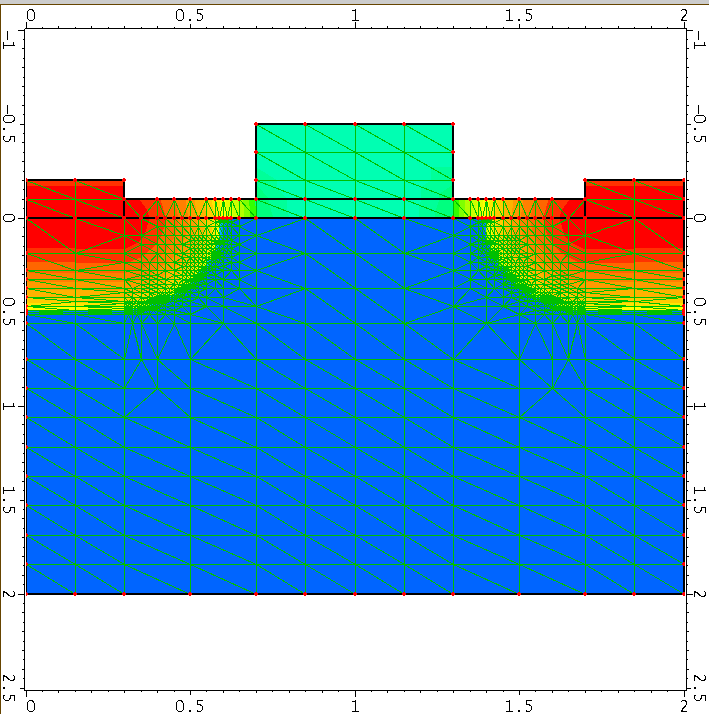
\includegraphics[width=0.6\textwidth]{img/nmos.png}
        \label{fig:nmos}}
        \hfil
        \subfigure[]{ 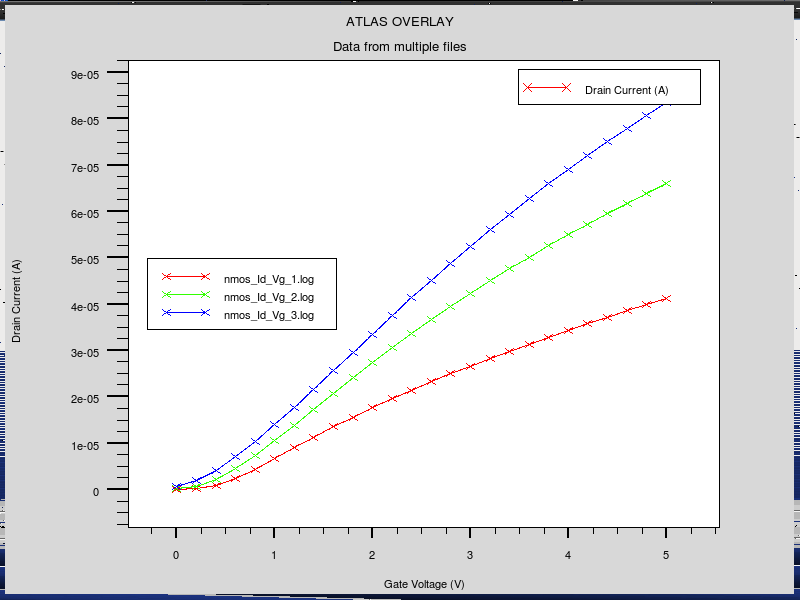
\includegraphics[width=0.4\textwidth]{img/nmos_Id_Vg.png}
        \label{fig:nmosVg}}
        \hfil
        \subfigure[]{ 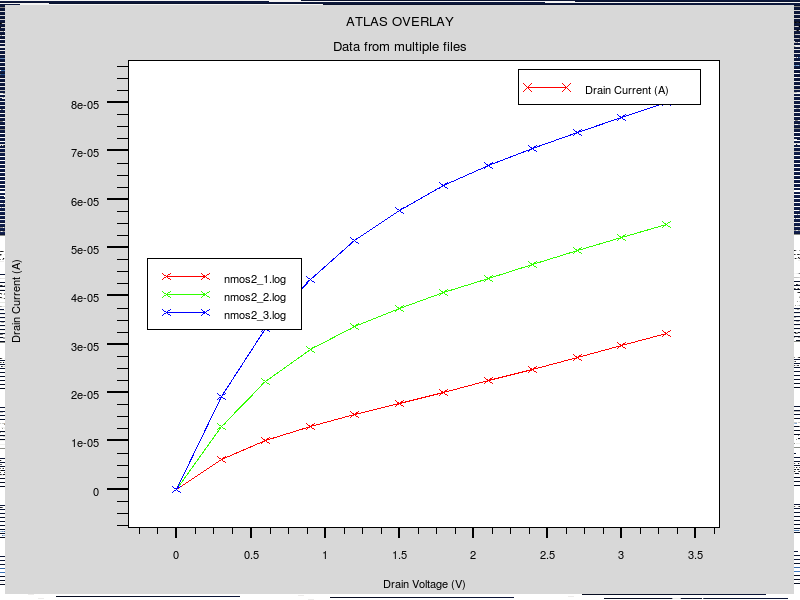
\includegraphics[width=0.4\textwidth]{img/nmos_Id_Vd.png}
        \label{fig:nmosVd}}
        \caption{(a)NMOS建模 (b)$I_d-V_g$特性曲线. (c)$I_d-V_d$特性曲线.}
    \end{figure} 

    \subsection{Devedit建模}
    利用Devedit对NMOS进行器件建模,如图\ref{fig:nmos}所示。
    
    \subsection{Atlas仿真}
    对NMOS进行仿真,得到$I_d-V_g$和$I_d-V_d$特性曲线,如图\ref{fig:nmosVg}和图\ref{fig:nmosVd}所示。

    
    \section{PMOS仿真}
    \begin{figure}[!h]
        \centering
        \subfigure[]{ 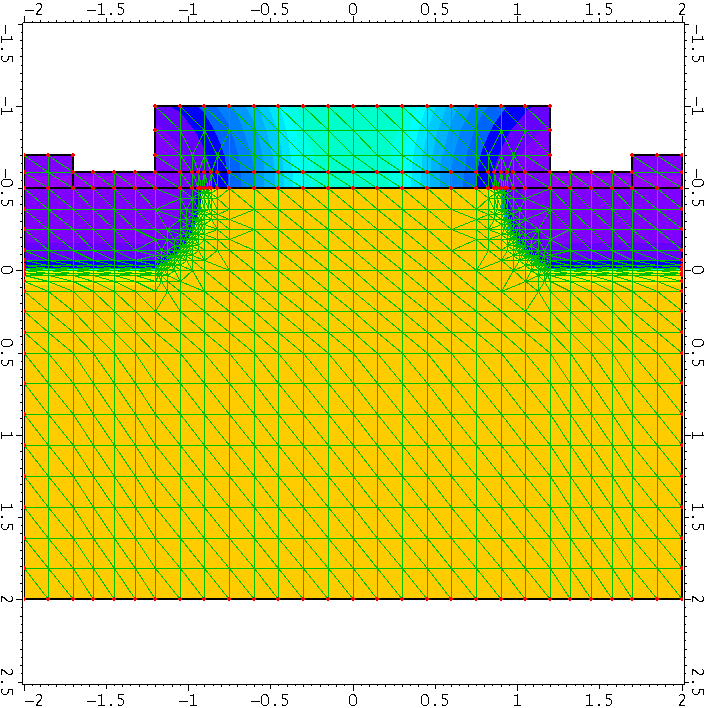
\includegraphics[width=0.6\textwidth]{img/pmos.png}
        \label{fig:pmos}}
        \hfil
        \subfigure[]{ 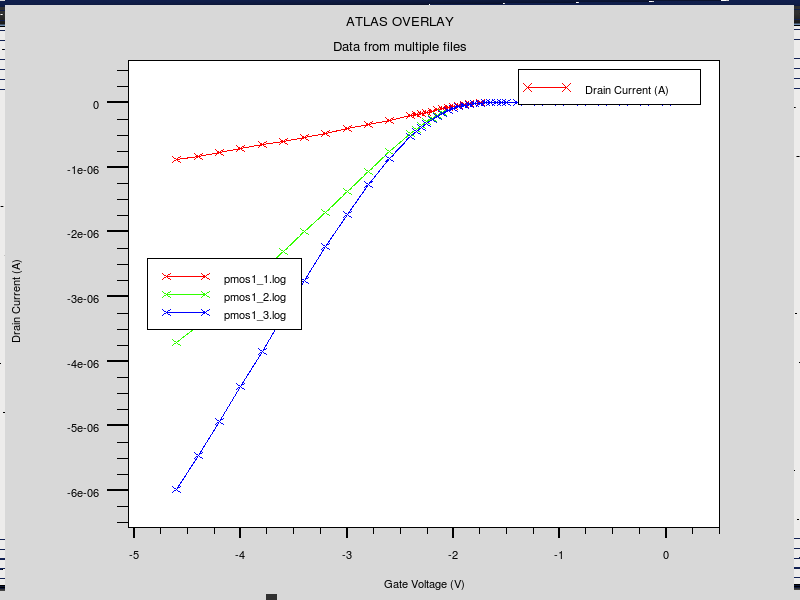
\includegraphics[width=0.4\textwidth]{img/pmos_Id_Vg.png}
        \label{fig:pmosVg}}
        \hfil
        \subfigure[]{ 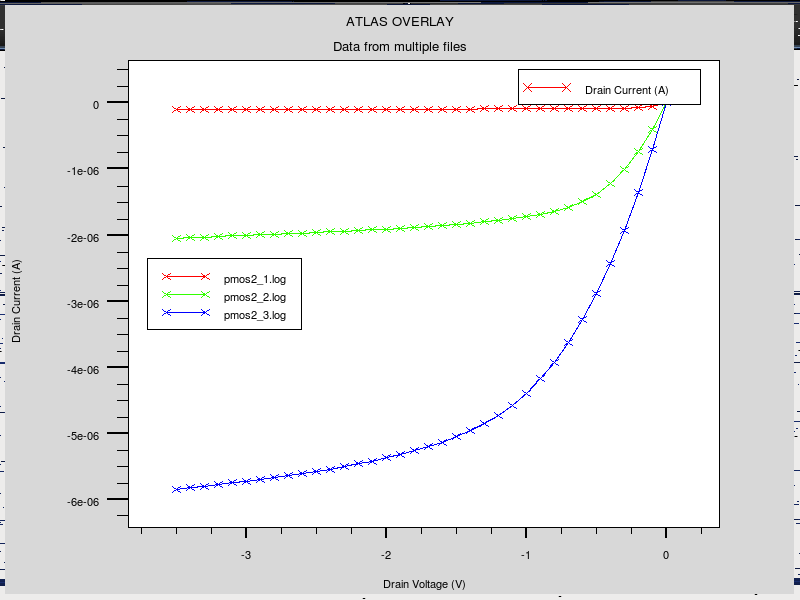
\includegraphics[width=0.4\textwidth]{img/pmos_Id_Vd.png}
        \label{fig:pmosVd}}
        \caption{(a)PMOS建模. (b)$I_d-V_g$特性曲线. (c)$I_d-V_d$特性曲线.}
    \end{figure}
    \subsection{Devedit建模}
    利用Devedit对PMOS进行器件建模,如图\ref{fig:pmos}所示。

    \subsection{Atlas仿真}
    对PMOS进行仿真,得到$I_d-V_g$和$I_d-V_d$特性曲线,如图\ref{fig:pmosVg}和图\ref{fig:pmosVd}所示。

    可见阈值电压$V_t$约为-1.5V。 影响$V_t$的因素有:
    金属功函数、衬底掺杂浓度、缺陷电荷、氧化层厚度等。

    \section{二极管仿真}
    \begin{figure}[!h]
        \centering
        \hfil
        \subfigure[]{ 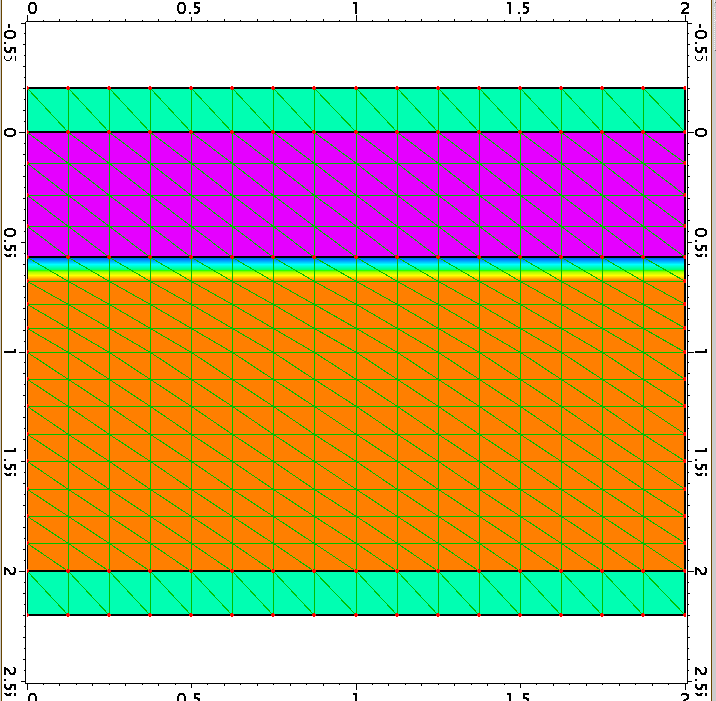
\includegraphics[width=0.5\textwidth]{img/diode.png}
        \label{fig:diode}}
        \newline
        \subfigure[]{ 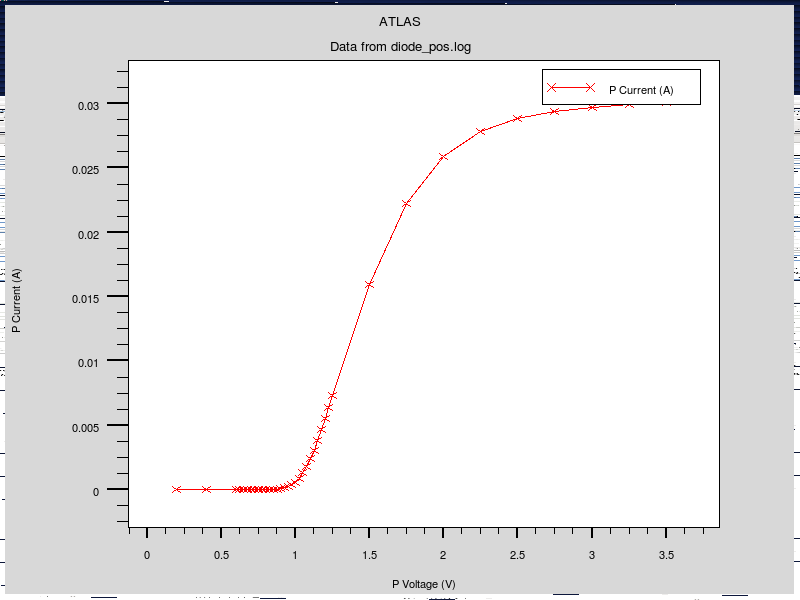
\includegraphics[width=0.4\textwidth]{img/diode_pos.png}
        \label{fig:pos}}
        \hfil
        \subfigure[]{ 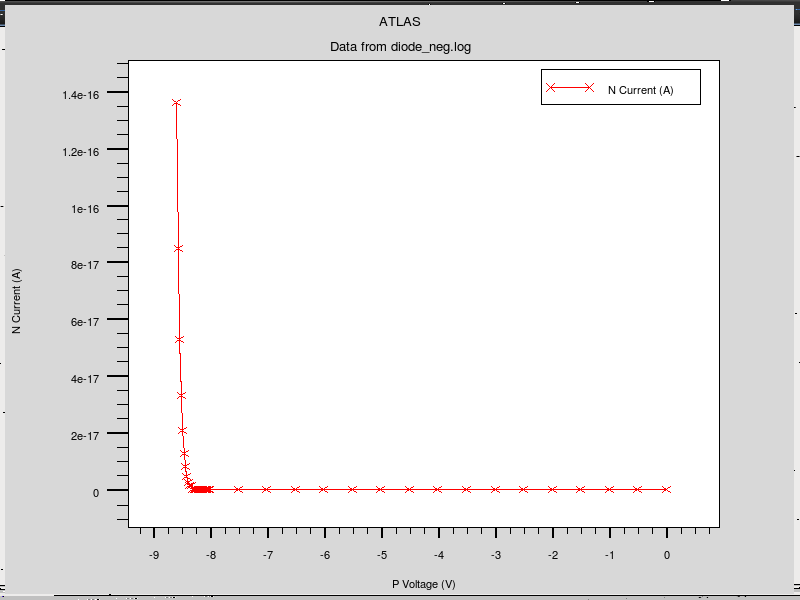
\includegraphics[width=0.4\textwidth]{img/diode_neg.png}
        \label{fig:neg}}
        \caption{(a)二极管建模. (b)二极管正向特性曲线. (c)二极管反向特性曲线.}
    \end{figure} 

    \subsection{Devedit建模}
    利用Devedit对二极管进行器件建模,如图\ref{fig:diode}所示。
 

    \subsection{Atlas仿真}
    对二极管进行仿真,得到正向和反向特性曲线,如图\ref{fig:pos}和图\ref{fig:neg}所示。

    
    
\end{document}

